\title{Event-Driven Architecture}
\author{Richard Thomas}
\date{\week{6}}

\maketitle

\section{Introduction}

Event-driven is an asynchronous architectural style.
It reacts to events, which is different to the common view of many designs which respond to requests.

Events provide a mechanism to manage asynchronous communication.
An event is sent to be handled, and the sender can continue with other tasks while the event is being processed.
If necessary, the handler can send a message back to the sender indicating the result of the event processing.

Each event handler can be implemented in its own independent execution environment.
This allows each type of handler to be easily scaled to handle its load.
Asynchronous communication means that event generators do not need to wait for the handler to process the event.
Handlers can generate their own events to indicate what they have done.
These events can be used to coordinate steps in a complex business process.

The service-based architecture example for the Sahara eCommerce system is designed to perform synchronous processing of requests.
A customer \emph{requests} to view a product's details through a REST API and receives a response with the result.
Similarly, a customer adding a product to their shopping cart is another request.

Adding auctions to the Sahara eCommerce system is a simple example that benefits from an event-driven architecture.
A customer sends a message to the Sahara eCommerce system initiating the \emph{event} of making a bid.
Upon receiving the bid event, the system checks the bid against the current high bid and determines the new high bid.
The system then generates a new high bid event.
This event triggers actions in the system to update the high bid and notify the bidder of the result of their bid.
It may also trigger an action to notify the previous high bidder that they are no longer the high bidder.

Multiple customers could submit bids for the same item at almost the same time (e.g. bid sniping).
These bid events are queued to be processed in the order they are received.
This queuing mechanism allows event handlers to process messages that arrive faster than the handler can process them.
It assumes that the message load will reduce in time and that the event handler will process all messages in the queue.

There are two basic approaches to implementing an event-driven architecture.
The terminology is that these are different \emph{topologies}, as they have different high-level structures.
The \emph{broker topology} is the simpler of the two and is optimised for performance, responsiveness, scalability, extensibility, and low coupling.
The \emph{mediator topology} is more complex but is designed to provide reliability, process control, and error handling.


\section{Broker Topology}

The broker topology consists of four elements.

\begin{description}
    \item[Initiating Event] starts the flow of events.
    \item[Event Broker] has \emph{channels} that receive events waiting to be handled.
    \item[Event Handler] accepts and processes events.
    \item[Processing Events] sent by an event handler when it has finished processing an event.
\end{description}

\begin{figure}[h!]
    \begin{adjustwidth}{-10mm}{-10mm}
        \centering
        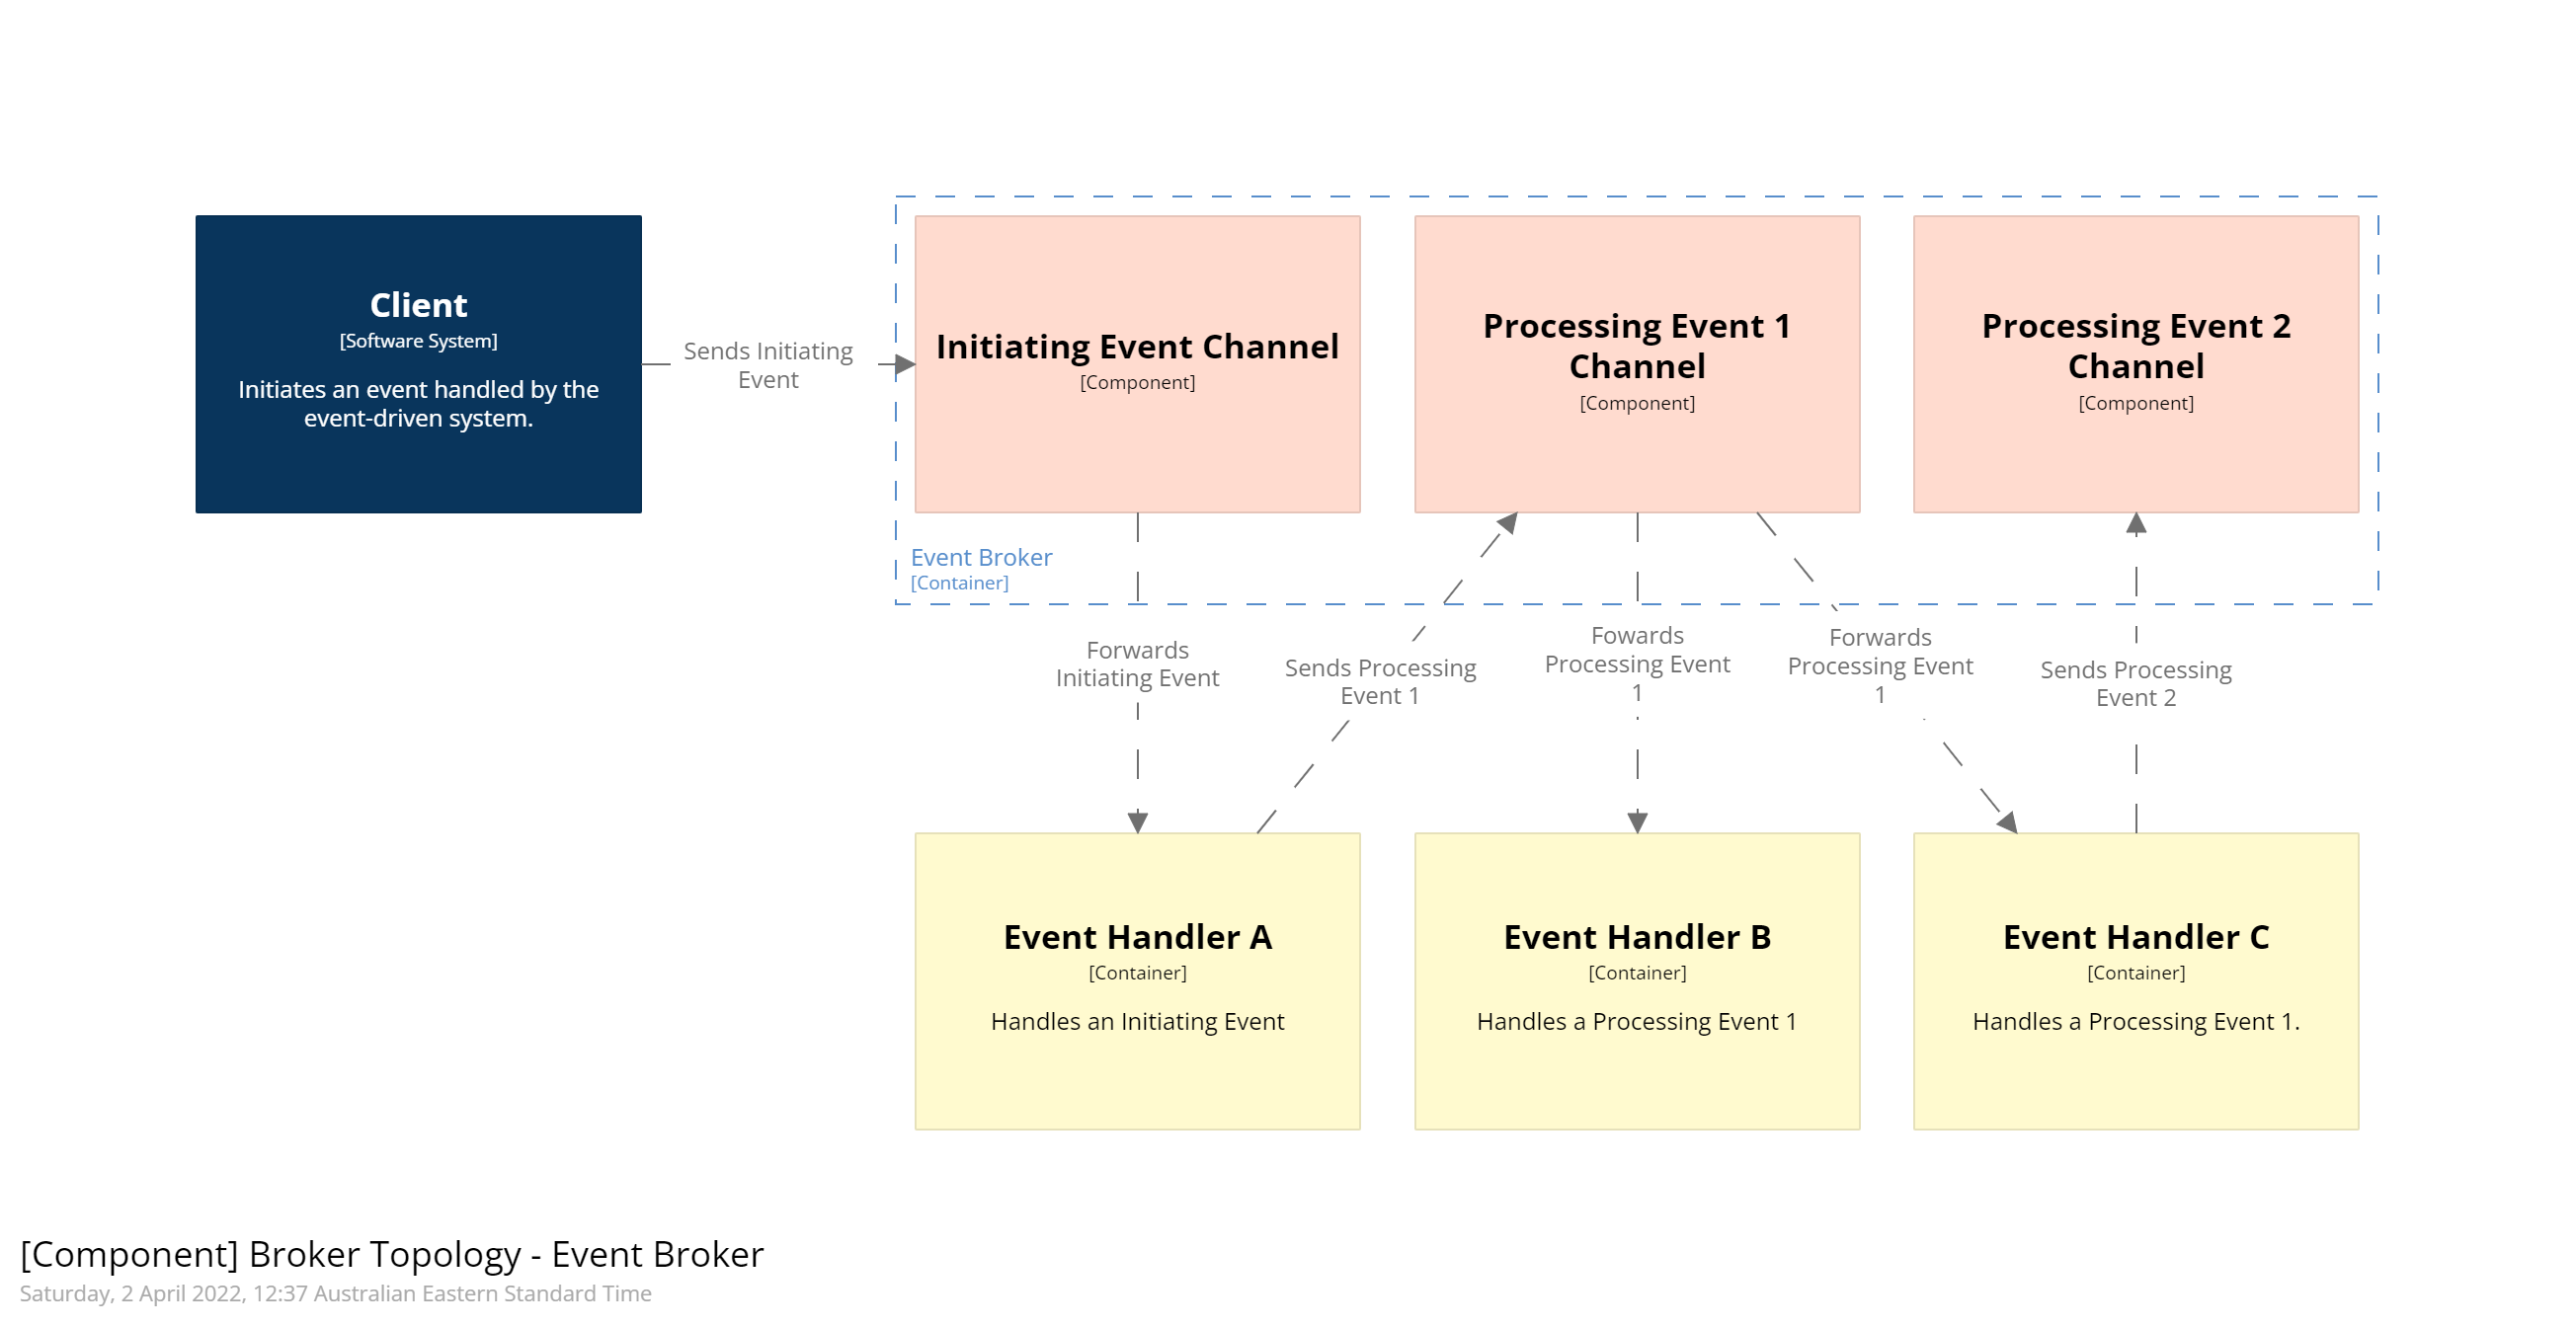
\includegraphics[trim=195 195 195 195,clip,width=0.97\paperwidth]{diagrams/broker-components.png}
    \end{adjustwidth}
    \caption{Basic broker topology.}
    \label{fig:broker-components}
\end{figure}

In figure \ref{fig:broker-components}, the \emph{Client} sends the \emph{Initiating Event} to the \emph{Initiating Event Channel} in the \emph{Event Broker}.
\emph{Event Handler A} accepts the event and processes it.
Upon completion of handling the \emph{Initiating Event},
\emph{Event Handler A} sends \emph{Processing Event 1} to the appropriate channel in the event broker.
Event handlers B and C accept this processing event and perform their actions.
When event handler C finishes processing it sends Processing Event 2 to its channel.
Event handler D accepts this event and performs its processing.


\section{Design Considerations}\label{sec:design-considerations}

A service-based architecture is typically used for medium-sized systems.


\section{Service-Based Principles}

There are a couple of principles which should be maintained when designing a service-based architecture
to produce a simple, maintainable, deployable and modular designs.

\vspace{1mm}
\begin{definition}[Independent Service Principle]\label{independent-service}
    Services should be independent, with no dependencies on other services.
\end{definition}



\section{Extensions}

There are a few common variations of the service-based architecture to consider.

\subsection{Separate Databases}

The first variation  we will consider is to have separate databases for each service.


\section{Conclusion}

Service-based architecture is an approach to designing a distributed system that is not too complex.
Domain services provide natural modularity and deployability characteristics in the architecture design.
Well designed service APIs improve the encapsulation and hide implementation details of the services.
